\section{Theoretische Grundlagen}
\label{sec:Theorie}
Zuerst betrachten wir wie es zur Dipolen in Ionenkristallen kommt und welche
Eigenschaften diese haben. Dazu betrachte man die Abbildung \ref{theo1}, es ist
ein Ionengitter mit einwertigen Ionen abgebildet (CsJ). Zur Erzeugung
der Dipole wird dieses Gitter mit $\text{Sr}^{2+}$ dotiert. Da der Kristall
elektrisch neutral ist, hat dieses eine Leerstelle zufolge. Es bildet
sich ein Dipol zuwischen dem dotierten Ion ($\text{Sr}^{2+})$ und der Leerstelle
mit einer Vorzugrichtung aus. Die so entstehenden Richtungen sind aufgrund
des Kristall diskretisiert.
\begin{figure}
\centering
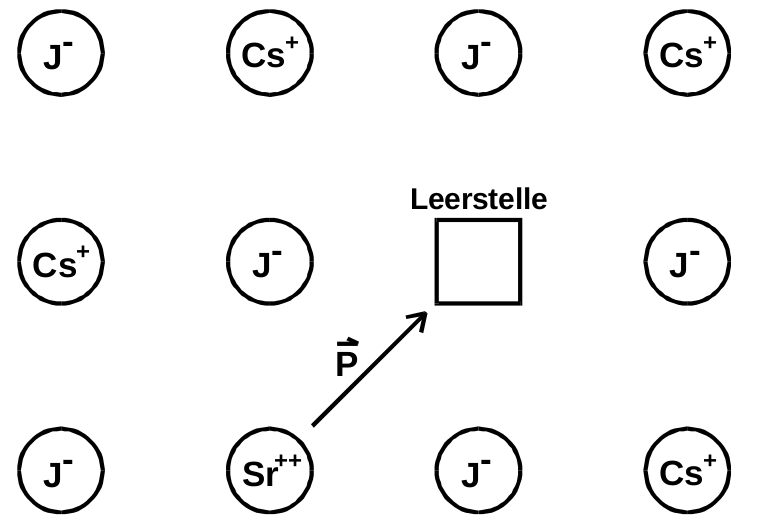
\includegraphics[width=0.8\textwidth]{ressources/ionengitter.png}
\caption{Darstellung eines Ionenkristallgitters mit einem ausgebildeten Dipol}
\label{theo1}
\end{figure}
Das Verhalten dieser Dipole hängt von der Temperatur des Kristalls ab. Für
Temperaturen unter $500°$C wird eine Änderung des Dipols nur über eine
Leerstellendiffusion erzeugt.
Diese kann nur statt finden, wenn eine materialspezifische Aktivierungsenergie
aufgebracht werden kann. Diese wird benötigt um die Änderung des Gitterpotentials
,welches durch die neue Konfiguration ensteht, zu ermöglichen. Die mittlere
Zeit die ein Dipol braucht, bis zwei Umorientierungen stattfinden bezeichnet man
als Relaxationzeit. Diese hängt davon ab wieviel des Gesamtdipolmomentes die Energie
$W$ bestitzt um die Potentialschwelle zu überwinden. Diese Größe ist
Boltzmann verteilt. Die Relaxationszeit ist gegeben durch:
$$
\tau(T)=\tau_0 \exp(\frac{W}{k_\text{B}T})
$$
Das $\tau_0$ wird als charakteristische Relaxationszeit bezeichnet und
gibt das Verhalten der Relaxationszeit im unendlichen an, sie ist
definiert als $\tau_0=\tau(\infty)$. Nach Definition der zu bestimmenden
Größen wird nun eine Betrachtung des Messverfahren durchgeführt.
\subsection{Messverfahren}
Zur Untersuchung der Dipole wird ein Plattenkondesator mit
Dielektrikum verwendet. Das Dielektrikum besitzt Dipole  die sich
ausrichten können. Hierzu wird ein elektrisches
Feld der Feldstärke $E$ angelegt. Dies führt zur einer Ausrichtung der
Dipole entlang des Feldes. Effekte wie die thermische Bewegungen des Gitters und
ähnliche Effekte führen dazu, dass sich nur ein Bruchteil der Dipole ausrichten kann.
Dieser Bruchteil $y$ lässt sich durch die Langevin-Funktion, welche ein
Funktion zur Berechnung von Orientierungspolarisationen ist, berechnen.
Sie ist gegeben durch:
$$y=L(x)=\coth(x)-1/x$$
Die Langevin-Funktion ist eine allgemeine Funktion, für den hier
betrachteten Fall lässt sich das $x$ identifizieren als
$$x=\frac{pE}{kT}.$$
Für das durchgeführte Experiment kann die Näherung getroffen werden das
$$pE \ll KT$$
sodass sich für die Langevin-Funktion ergibt:
$$y(T)=\frac{pE}{3kT}$$
Zusätzlich muss angenommen werden, dass Dipole lange gegenüber der
Relaxationzeit im E-Feld aufhalten. Damit die obenstehende Gleichung
gilt.

\begin{figure}
\centering
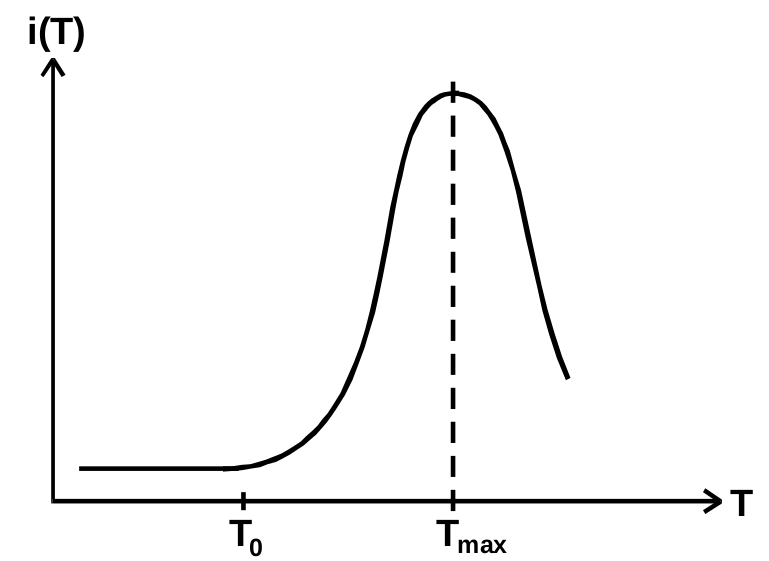
\includegraphics[width=0.8\textwidth]{ressources/stromfluss.png}
\caption{Darstellung eines Ionenkristallgitters mit einem ausgebildeten Dipol}
\label{theo1}
\end{figure}


% 2x2 Plot
% \begin{figure*}
%     \centering
%     \begin{subfigure}[b]{0.475\textwidth}
%         \centering
%         \includegraphics[width=\textwidth]{Abbildungen/Schaltung1.pdf}
%         \caption[]%
%         {{\small Schaltung 1.}}
%         \label{fig:Schaltung1}
%     \end{subfigure}
%     \hfill
%     \begin{subfigure}[b]{0.475\textwidth}
%         \centering
%         \includegraphics[width=\textwidth]{Abbildungen/Schaltung2.pdf}
%         \caption[]%
%         {{\small Schaltung 2.}}
%         \label{fig:Schaltung2}
%     \end{subfigure}
%     \vskip\baselineskip
%     \begin{subfigure}[b]{0.475\textwidth}
%         \centering
%         \includegraphics[width=\textwidth]{Abbildungen/Schaltung4.pdf}    % Zahlen vertauscht ... -.-
%         \caption[]%
%         {{\small Schaltung 3.}}
%         \label{fig:Schaltung3}
%     \end{subfigure}
%     \quad
%     \begin{subfigure}[b]{0.475\textwidth}
%         \centering
%         \includegraphics[width=\textwidth]{Abbildungen/Schaltung3.pdf}
%         \caption[]%
%         {{\small Schaltung 4.}}
%         \label{fig:Schaltung4}
%     \end{subfigure}
%     \caption[]
%     {Ersatzschaltbilder der verschiedenen Teilaufgaben.}
%     \label{fig:Schaltungen}
% \end{figure*}
